%----------------------------------------------------------------------------------------
% Tiro parabólico
%----------------------------------------------------------------------------------------

Esta práctica se hará uso de \emph{regresión polinomial} para inferir el tipo de curva que describe mejor el movimiento de un objeto al ser lanzado.


\section{Objetivo}

Que el alumno aplique la \textit{regresión polinomial} para encontra la ecuación que describe fenómeno físico.  Utilzará conjuntos de entrenamiento, validación y prueba para seleccionar la familia de hipótesis correcta, que no se sobreajuste (\textit{overfitting}) a los datos ni tenga un ajuste pobre (\textit{underfitting}).

\begin{auxcode}
 \caption{Regresión polinomial}
 \centering
 \hurl{\auxprefix ia-regresion-logistica}
\end{auxcode}



\section{Introducción}

\subsection{Tiro parabólico}

\noindent El problema del tiro parabólico es ampliamente conocido en el área de la física: un objeto es lanzado con un cierto ángulo y, mientras avanza, es atraído por la gravedad, de tal forma que también cae.  La ecuación que describe tal movimiento en su forma paramétrica es:
\begin{align*}
 P(t) &=
 \begin{bmatrix}
  x(t) \\
  y(t)
 \end{bmatrix}
 =
 \begin{bmatrix}
  x_0 + v_{0}\cos(\alpha) t \\
  y_0 + v_{0}\sin(\alpha) t - \frac{1}{2}gt^2
 \end{bmatrix}
\end{align*}

De estas ecuaciones es posible despejar el tiempo al cual la pelota llegará a la altura cero:
\begin{align*}
  t_f &= \dfrac{v_{0}\sin\alpha + \sqrt{(v_{0}\sin\alpha)^2 + 2g y_0}}{g}
\end{align*}

La ecuación que describe la curva geométrica que se obtiene es entonces una parábola de la forma:
\begin{align*}
 y &= c + bx + ax^2
\end{align*}


Es posible estudiar este movimiento en detalle haciendo uso de un estroboscopio y una cámara.  Para captar la posición de una pequeña pelota, que es lanzada a cierto ángulo, se le toma una foto manteniendo el obturador abierto todo el tiempo que dura el movimiento, pero la escena sólo es iluminada por el estroboscopio que emite luz a una frecuencia conocida.  El resultado es una foto donde la pelota aparece a intervalos regulares en las diferentes posiciones que fue ocupando a lo largo de su trayetoria.  El obturador se debe abrir al lanzar la pelota y cerrar cuando esta regresa a la altura de la cual fue lanzada.  \fref{fig:tiropelota}

\begin{figure}
 \centering
 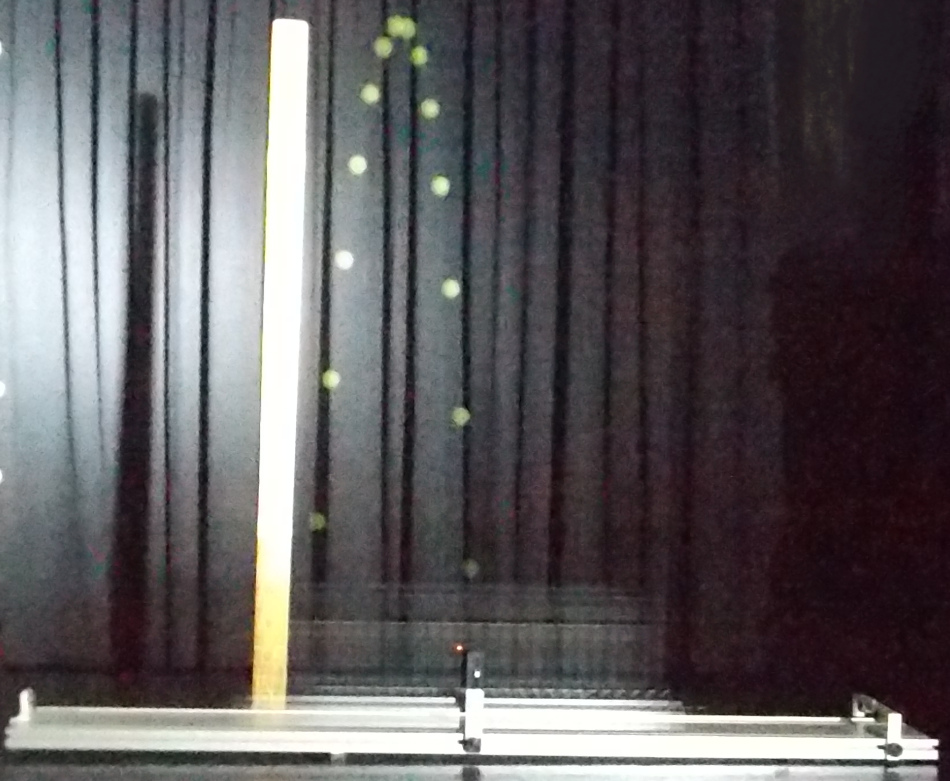
\includegraphics[width=0.5\textwidth]{regresionpoli/fis_carritoBalistico_peque.jpg}
 \caption{Agradecemos al laboratorio de mecánica de la Facultad de Ciencias por proporcionarnos la foto.}\label{fig:tiropelota}
\end{figure}

Dado que conocemos la ecuación que describe este movimiento, podemos proceder a probar la técnica de regresión polinomial generando datos artificiales.  El procedimiento consiste en generar muestras a partir del tiempo $t=0$, cada intervalo $\Delta t$, de modo que los valores obtenidos para $x$ y $y$ simulen las posiciones de la pelota en los tiempos $\{0, \Delta t, 2 \Delta t, ..., t_f\}$.  Al realizar este procedimiento se obtiene una gráfica como la de la \fref{fig:muestras}.

\begin{figure}
 \centering
 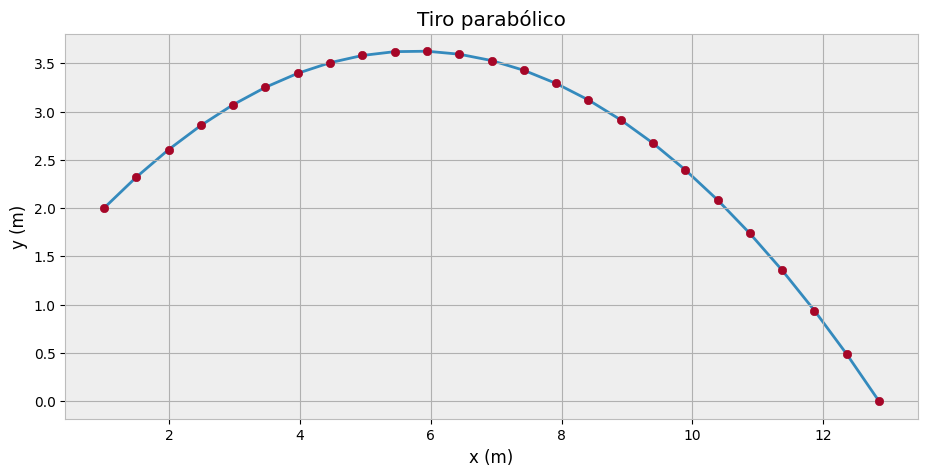
\includegraphics[width=0.7\textwidth]{regresionpoli/muestras}
 \caption{Muestreo regular de la ecuación de tiro parabólico.}\label{fig:muestras}
\end{figure}

Sin embargo, de realizarse las mediciones sobre la fotografía del fenómeno real, existiría un cierto margen de error, que haría que las mediciones no cayeran exactamente sobre la parábola.  Para simular este fenómeno agregaremos ruido Gaussiano a los valores obtenidos.  Esto se logra remuestreando las coordenadas $(x,y)$.  Para cada coordenada se generará un par nuevo tomando una muestra de la distribución Gaussiana que tiene como media a cada componente del par coordenado.  Recordemos que la función Gaussiana está dada por:
\begin{align*}
f(x|\mu=0, \sigma=1) = \frac{1}{\sqrt{2 \pi \sigma^2}} e^{-\frac{(x - \mu)^2}{2 \sigma^2}}
\end{align*}
y tiene la forma de una campana con centro en $\mu$.  La probabilidad de que la muestra se encuentre más cerca del valor original o más lejos se ve afectada por la desviación estándar $\sigma$, que determina el ancho de la campana []\fref{fig:campana}].

\begin{figure}
 \centering
 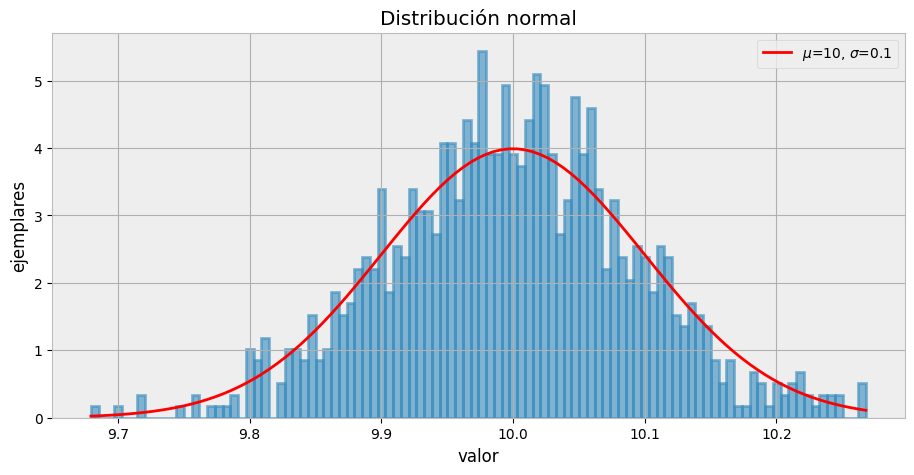
\includegraphics[width=0.7\textwidth]{regresionpoli/normal}
 \caption{Muestreo regular de la ecuación de tiro parabólico.}\label{fig:campana}
\end{figure}

De este modo, al remuestrear los puntos de la parábola, utilizando la distribución Gaussiana, obtendremos un nuevo conjunto, como el mostrado en \fref{fig:muestrasruido}.
\begin{figure}
 \centering
 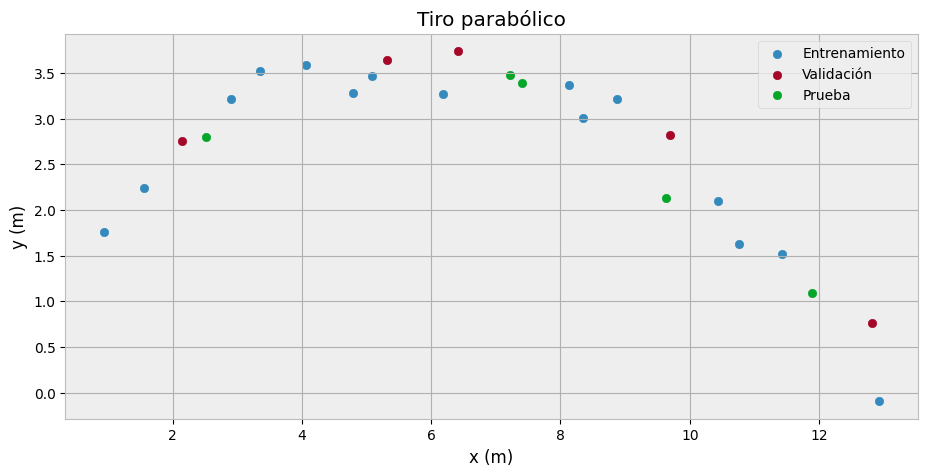
\includegraphics[width=0.7\textwidth]{regresionpoli/muestrasruido}
 \caption{Muestreo de la ecuación de tiro parabólico a partir de la distribución Gaussiana con $\sigma=0.2$.  Las muestras han sido asignadas aleatoriamente a los conjuntos de entrenamiento, validación y prueba.}\label{fig:muestrasruido}
\end{figure}
Claramente los errores de medición inducidos en esta imagen son algo exagerados, pero servirán para poner a prueba las técnicas siguientes.  Si se quiere una simulación más realista basta con reducir el valor de $\sigma$.



\subsection{Regresión polinomial}

El caso del tiro parábolico es un caso especial: sólo tenemos dos variables $x$ y $y$.  Gracias a ello podemos graficar nuestras mediciones y ver que es posible ajustar una parábola a los datos.  En los conjuntos de datos que se analizan actualmente hay decenas o cientos de variables y no es posible visualizar directamente cómo se relacionan estos datos, por lo que se requieren técnicas que permitan seleccionar la ecuación que mejor describe a los datos y permite hacer predicciones basándose únicamente en criterios numéricos.  De este modo, utilizaremos el ejemplo del tiro parabólico, que podemos ver, para darnos una idea de cómo se comportan los métodos diseñados para cuando no se puede.

Supongamos entonces que no sabemos cuál es la curva que se puede ajustar a estos datos, pero tenemos información que sugiere que puede tratarse de algún polinomio.  Procedemos a proponer \emph{espacios de hipótesis} que podrían ajustarse a los datos.  Un ejemplo de espacio de hipótesis es la familia de las rectas:
\begin{align*}
h_{\Theta}(x) &= \theta_0 + \theta_1 x
\end{align*}
Dado un conjunto de datos, deseamos encontrar la hipótesis que se ajusta mejor a estos datos y predice mejor las respuestas para datos no vistos.  Esta hipótesis estará dada por valores concretos de los parámetros $\theta_0$ y $\theta_1$.  Para encontrarla se elige aquella cuyos errores sobre el conjunto de entrenamiento sean menores.  Su capacidad de predicción se evalúa con el conjunto de validación.

Sin embargo ¿qué sucede si ninguna recta puede describir correctamente nuestros datos? Es decir, si el error siguie siendo demasiado alto.  De hecho, en este caso, claramente un recta es demasiado sencilla para describir el movimiento de la pelota, los errores cometidos por cualquier recta serán siempre grandes.  Tenemos un caso de \emph{ajuste pobre}.

Tendríamos que proponer otro espacio de hipótesis.  Por ejemplo, el espacio de las parábolas.
\begin{align*}
 h_{\Theta}(x) &= \theta_0 + \theta_1 x + \theta_2 x^2
\end{align*}
Ahora hay tres parámetros que ajustar, es decir, contamos con tres \emph{grados de libertad}.  Para el tiro parabólico sabemos que este espacio sí contiene la respuesta correcta.  Pero supongamos que no lo sabemos.  Tendremos que probar con otros espacios: polinomios cúbicos, cuarta potencia, etc. y no sólo elegir una hipótesis dentro de cada espacio posible, sino elegir qué espacio es el más adecuado.

Mediremos el error que comete cada hipótesis con la función:
\begin{align*}
Error &= \frac{1}{2m} \sum_{i=1}^{m} (h_{\Theta}(x^{(i)})-y^{(i)})^2
\end{align*}
Es posible despejar los parámetros que llevan el gradiente de esta función de error a cero, obteniédose una fórmula general para encontrar los coeficientes del polinomio optimo para el grado $n$.  Sea la hipótesis:
\begin{align*}
 h_\theta(x) &= \theta_0 x_0 + \theta_1 x_1 + \theta_2 x_2 + ... + \theta_n x_n \\
 x_0 &\equiv 1
\end{align*}
en forma matricial:
\begin{align*}
 h_\theta(x) &= \Theta^T X = X^T \Theta
\end{align*}
con
\begin{align}
\mat{X} &= \begin{bmatrix}
       x_0^{(1)} x_1^{(1)} ... x_n^{(1)}  \\
       x_0^{(2)} x_1^{(2)} ... x_n^{(2)}  \\
       ...\\
       x_0^{(m)} x_1^{(m)} ... x_n^{(m)}
      \end{bmatrix} &
  \Theta &= \begin{bmatrix}
             \theta_0 \\
             \theta_1 \\
             ... \\
             \theta_n
            \end{bmatrix} &
  Y &= \begin{bmatrix}
       y_0 \\
       y_1\\
       ...\\
       y_n
      \end{bmatrix}
\end{align}
La ecuación normal que calcula los parámetros óptimos es:
\begin{align}
\Theta &= (\mat{X}^T \mat{X})^{-1} \mat{X}^T Y
\end{align}
La complejidad para el cálculo de esta fórmula es $\mathcal{O}(n^3)$.  Mientras $n$ no sea demasiado grande se puede usar.

Ahora, hay otro problema: entre más grados de libertad considere el espacio de hipóptesis, mayor capacidad tendrá para ajustarse a los datos entrenamiento, decimos que el espacio es más \textit{expresivo}.  Esto quiere decir que, a mayor número de grados de libertad, menor será el error en el conjunto de entrenamiento.  Pareciera entonces que la mejor hipótesis es la que utiliza más grados de libertad, pero esto no es así, porque entre más se ajusta a los datos de entrenamiento, peor se irá comportando al momento de predecir las respuestas para valores no vistos, esto es un \emph{sobreajuste}.  El mejor espacio de hipótesis será el que ofrezca la hipótesis con los mejores resultados en el conjunto de validación, es decir, la que haga mejores predicciones.  La \fref{fig:variosajustes} muestra qué sucede al ajustar polinomios de grado creciente a los datos del tiro parabólico.


\begin{figure}
 \centering
 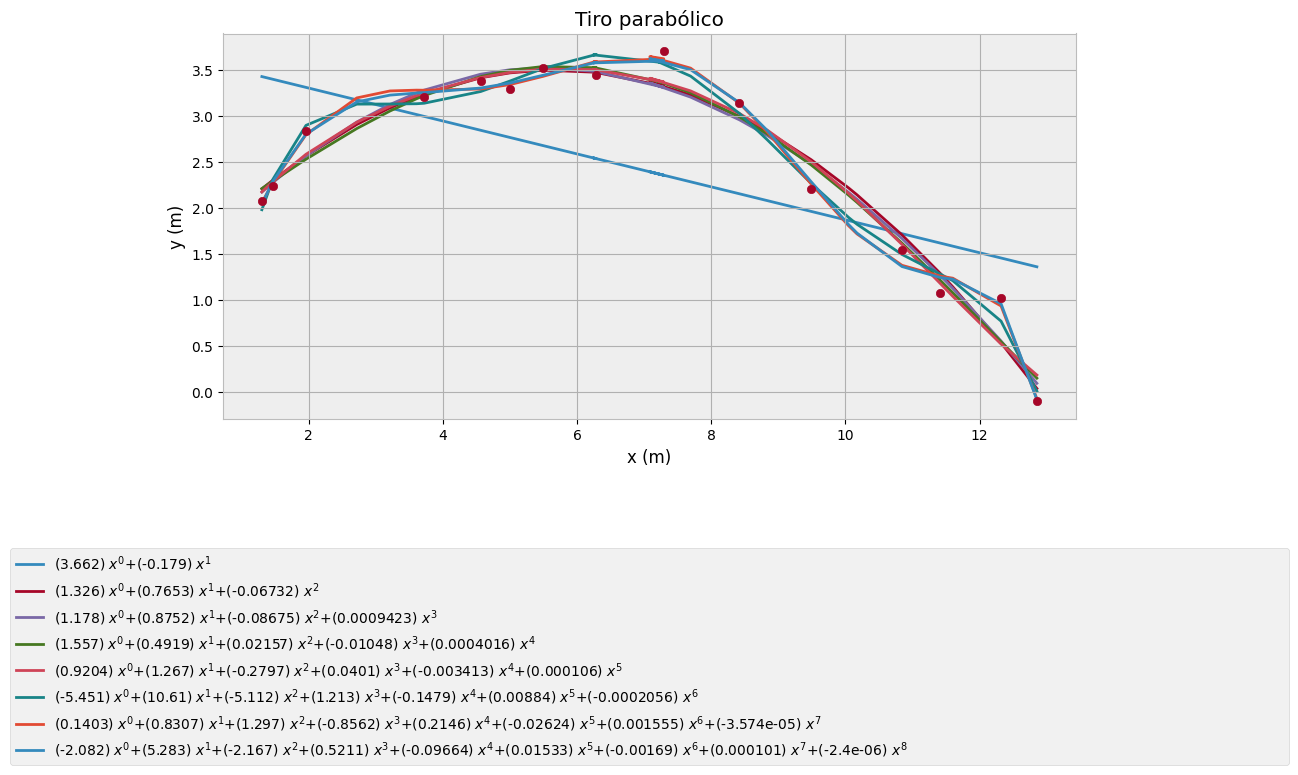
\includegraphics[width=\textwidth]{regresionpoli/variosajustes}
 \caption{Ajuste de polinomios de grado creciente a los datos de entrenamiento.  Entre más grande es el grado más oscila el polinomio, pasando cada vez más cerca de los datos de entrenamiento, pero despegándose de la curva descrita por la pelota.}\label{fig:variosajustes}
\end{figure}


Una estrategia para eligir a la mejor hipótesis es graficar el error en el conjunto de entrenamiento y de validación para cada grado probado y observar el mínimo en la curva error en validación vs grado.  A ese punto se le llama coloquialmente el \textit{codo}.  Ese será el grado para la hipótesis elegida.

\begin{figure}
 \centering
 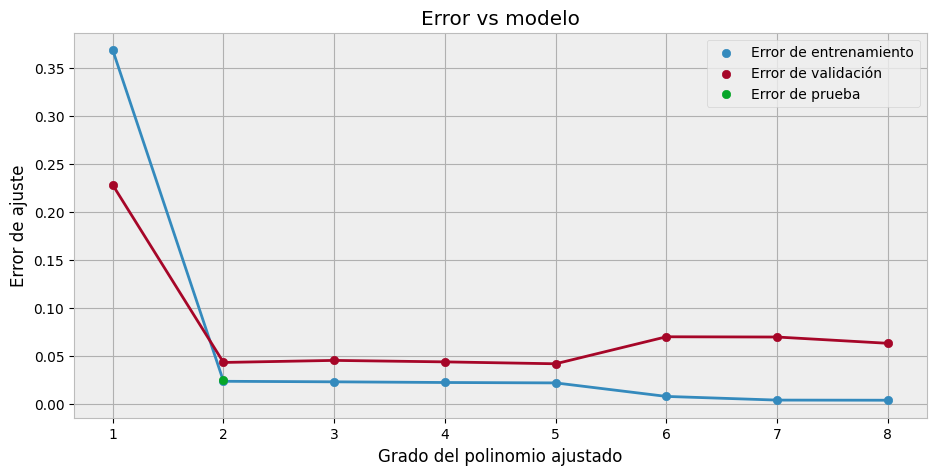
\includegraphics[width=\textwidth]{regresionpoli/codopolinomios}
 \caption{Ajuste de polinomios de grado creciente a los datos de entrenamiento.  Entre más grande es el grado más oscila el polinomio, pasando cada vez más cerca de los datos de entrenamiento, pero despegándose de la curva descrita por la pelota.}\label{fig:codopolinomios}
\end{figure}

Una vez que se eligió un espacio de hipótesis y una hipótesis dentro de este, se usa el conjunto de prueba para estimar el comportamiento de la hipótesis elegida ante datos que no se usaron durante ninguna elección en el proceso que llevó a su selección.


\subsection{Regularización}

En el caso de las curvas polinomiales es sencillo generar esta gráfica error vs grado; pero para otras familias de espacios de hipótesis no será tan sencillo, por ejemplo, para redes neuronales donde se pueden considerar conexiones entre miles o millones de neuronas.  Por ello se diseñó una técnica semejante que prueba la suma de todas las hipótesis al mismo tiempo y forza a que el proceso de minimización de la función de error de más peso a los términos más relevantes.  Esta técnica es la \emph{regularización}, que agrega un término a la función de error para indicar qué tanta expresividad se permitirá otorgar al espacio de hipótesis.

Por ejemplo, la siguiente de pérdida es la suma del error original y regularización **L2**, que incrementa el valor de la pérdida cuando la magnitud de los parámetros crece:
\begin{align}
 \mathcal{L} &= \frac{1}{2m} \sum_{i=1}^{m} (h_{\Theta}(x^{(i)})-y^{(i)})^2 + \lambda \Theta^T\Theta
\end{align}

La nueva forma normal vectorizada, que resuelve el problema de minimización, se ve como:
\begin{align}
 \Theta &= (\mat{X}^T \mat{X} + \lambda \mat{K})^{-1}\mat{X}^T Y
\end{align}

Para minimizar $\mathcal{L}$ la hipótesis deberá incrementar la magnitud de los parámetros que acompañan a los términos que ayudan más a predecir la respuesta correcta, mientras que reduce los de aquellos términos que no ayudan tanto.  El valor de $\lambda$ indica qué tanto podrán crecer los coeficientes $\theta_i$.  Un valor grande de $\lambda$ produce una penalización muy fuerte, por lo que se podrán usar pocos términos; es algo semejante a usar polinomios con grados pequeños.  Un valor pequeño de $\lambda$ casi no aplica penalización por lo que todos los términos son considerados; es semejante a tener un polinomio de grado alto con todos sus términos.  De este modo, ahora se requiere elegir la magnitud adecuada de $\lambda$ para obtener la hipótesis que haga mejores predicciones.  Para ello también se puede utilizar la técnica del codo. [\fref{fig:codolambda}]

\begin{figure}
 \centering
 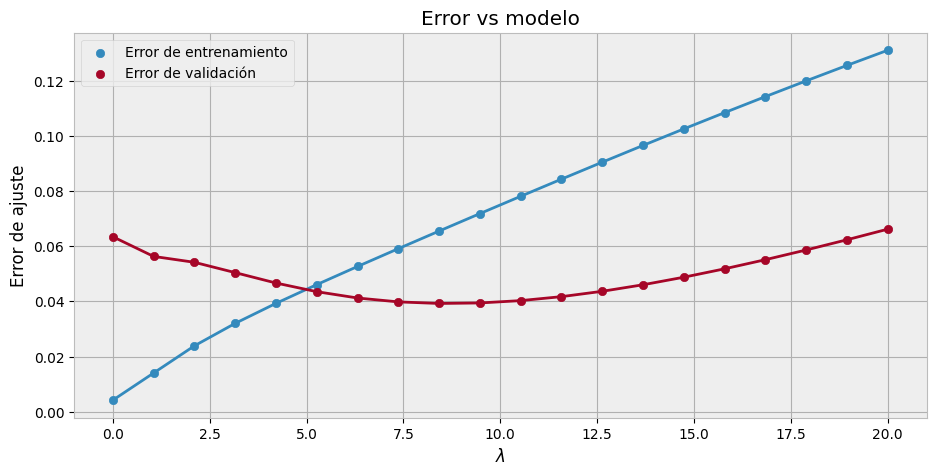
\includegraphics[width=\textwidth]{regresionpoli/codolambda}
 \caption{El error mínimo en el conjunto de validación se da para $\lambda=8.42$, por lo que se elige la hipótesis que resuelve la ecuación normal con ese valor de $\lambda$.}\label{fig:codolambda}
\end{figure}




\section{Desarrollo e implementación}

Para esta práctica deberás reproducir el experimento simulado del tiro parabólico.  Se recomienda crear un cuaderno de \Python y usar \code{matplotlib} para generar las gráficas.

\begin{enumerate}
 \item Genera muestras del tiro parabólico a partir de la ecuación paramétrica.
 \item Utiliza la distribución Gaussiana para muestrear datos que simulen mediciones con ruido.
 \item Divide tus datos aleatoriamente en conjuntos de entrenamiento (70\%), validación (20\%) y prueba (\%10).
 \item Realiza el entrenamiento para polinomios de grados desde uno hasta ocho.
 \item Genera la gráfica error vs grado tanto en el conjunto de entrenamiento como en el de validación. Reporta el resultado obtenido, especialmente cuál fue el modelo seleccionado y cuál es su error en el conjunto de prueba.
 \item Repite el procediento usando regularización. Reporta el resultado obtenido.
\end{enumerate}



\section{Requisitos y resultados}

La implementación de las técnicas anteriores deberá realizarse de forma genérica, es decir, deberán generarse datos para cualquier tiro parabólico dados los parámetros correspondientes y no sólo un ejemplar.  En función de estos parámetros deberá generarse una visualización de los datos en una gráfica 2D.  Igualmente es obligatorio generar las gráficas de error vs grado para los conjuntos de entrenamiento y validación.
